\title[High-frequency switching cell]{The high-frequency switching cell}
\section{High-frequency switching cell}

\begin{frame}[plain]
	\titlepage
\end{frame}

%%%%%%%%%%%%%%%%%%%%%%%%%%%%%%%%%%%%%%%%%%%%%%%%%%%%%%%%%%%%%
%% Overview %%
%%%%%%%%%%%%%%%%%%%%%%%%%%%%%%%%%%%%%%%%%%%%%%%%%%%%%%%%%%%%%
\subsection{Recap from PEDC}

\begin{frame}
	\frametitle{Overview}
	Lecture 1 showed that switching losses grow with $f_\mathrm{sw}$ while conduction loss does not. This lecture looks at the first rung of the frequency ladder in detail: the losses of the switching cell itself.
	\begin{itemize}
		\item Recap: switching transitions and figures of merit (PEDC L05--L06)
		\item The output capacitance: charge, energy and hysteresis
		\item The complete loss inventory of a switching cell at MHz
		\item Hard versus soft switching and the optimum die size
		\item Device technologies and packages for high frequency
	\end{itemize}
	After this lecture you can set up a loss budget from datasheet values and choose a device for a given voltage, current and switching frequency.
\end{frame}

%%%%%%%%%%%%%%%%%%%%%%%%%%%%%%%%%%%%%%%%%%%%%%%%%%%%%%%%%%%%%
%% Switching transitions %%
%%%%%%%%%%%%%%%%%%%%%%%%%%%%%%%%%%%%%%%%%%%%%%%%%%%%%%%%%%%%%
\begin{frame}
	\frametitle{Hard turn-on transition}
	\begin{columns}[T]
		\begin{column}{0.5\textwidth}
			\begin{figure}
				\centering
				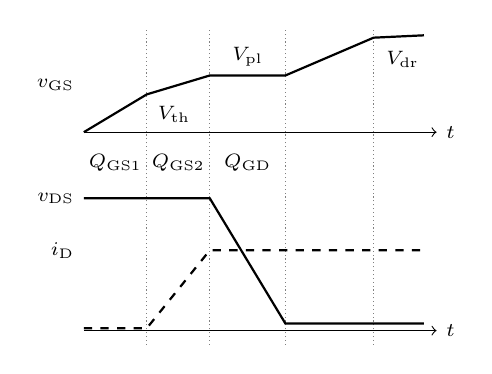
\begin{tikzpicture}[x=0.8cm, y=0.6cm, font=\scriptsize]
					% time markers
					\foreach \t in {1,2,3.2,4.6} {\draw[densely dotted, gray] (\t,-3.3) -- (\t,3.4);}
					% gate-source voltage
					\draw[->] (0,1.2) -- (5.6,1.2) node[right] {$t$};
					\draw[thick] (0,1.2) -- (1,2.0) -- (2,2.4) -- (3.2,2.4) -- (4.6,3.2) -- (5.4,3.25);
					\node[anchor=east] at (0,2.2) {$v_\mathrm{GS}$};
					\node[anchor=west] at (4.65,2.75) {$V_\mathrm{dr}$};
					\node[anchor=south] at (2.6,2.4) {$V_\mathrm{pl}$};
					\node[anchor=north west] at (1.02,1.95) {$V_\mathrm{th}$};
					% drain current and drain-source voltage
					\draw[->] (0,-3) -- (5.6,-3) node[right] {$t$};
					\draw[thick] (0,-0.2) -- (2,-0.2) -- (3.2,-2.85) -- (5.4,-2.85);
					\draw[thick, dashed] (0,-2.95) -- (1,-2.95) -- (2,-1.3) -- (5.4,-1.3);
					\node[anchor=east] at (0,-0.2) {$v_\mathrm{DS}$};
					\node[anchor=east] at (0,-1.3) {$i_\mathrm{D}$};
					% intervals
					\node at (1.5,0.55) {$Q_\mathrm{GS2}$};
					\node at (2.6,0.55) {$Q_\mathrm{GD}$};
					\node at (0.5,0.55) {$Q_\mathrm{GS1}$};
				\end{tikzpicture}
				\caption{Clamped inductive turn-on (simplified: no ringing, no reverse recovery)}
			\end{figure}
		\end{column}
		\begin{column}{0.47\textwidth}
			With the total gate resistance $R_\mathrm{G}$ (driver, external and internal):
			\begin{align*}
				t_\mathrm{ir} & \approx \frac{R_\mathrm{G}\,Q_\mathrm{GS2}}{V_\mathrm{dr}-V_\mathrm{pl}}, \quad
				t_\mathrm{vf} \approx \frac{R_\mathrm{G}\,Q_\mathrm{GD}}{V_\mathrm{dr}-V_\mathrm{pl}} \\
				E_\mathrm{on} & \approx \tfrac{1}{2}V_\mathrm{DC}I_\mathrm{L}(t_\mathrm{ir}+t_\mathrm{vf}) \\
				              & \quad + Q_\mathrm{oss}V_\mathrm{DC} + Q_\mathrm{rr}V_\mathrm{DC}
			\end{align*}
			For the turn-off transition with the driver at 0\,V, replace $V_\mathrm{dr}-V_\mathrm{pl}$ by $V_\mathrm{pl}$.\\[0.4em]
			{\small The charges $Q_\mathrm{GS2}$ and $Q_\mathrm{GD}$ set the overlap time, the charges $Q_\mathrm{oss}$ and $Q_\mathrm{rr}$ add a loss that no gate driver can remove.}
		\end{column}
	\end{columns}
	\blfootnote{Details: PEDC L05 (MOSFET switching) and L06 (WBG devices).}
\end{frame}

%%%%%%%%%%%%%%%%%%%%%%%%%%%%%%%%%%%%%%%%%%%%%%%%%%%%%%%%%%%%%
%% Figures of merit %%
%%%%%%%%%%%%%%%%%%%%%%%%%%%%%%%%%%%%%%%%%%%%%%%%%%%%%%%%%%%%%
\begin{frame}
	\frametitle{Figures of merit}
	\begin{table}
		\centering
		\small
		\begin{tabular}{|l|>{\raggedright\arraybackslash}p{4.3cm}|>{\raggedright\arraybackslash}p{4.6cm}|}
			\hline
			\textbf{Figure of merit}                                 & \textbf{Compares}                       & \textbf{Relevant for}                                  \\
			\hline
			$R_\mathrm{DS(on)}\,Q_\mathrm{G}$                        & conduction and gate-drive loss          & all converters, gate driver sizing                     \\
			$R_\mathrm{DS(on)}\,(Q_\mathrm{GD}+Q_\mathrm{GS2})$      & conduction and $V$--$I$ overlap loss    & hard switching ($\mathrm{FOM_{HS}}$)                   \\
			$R_\mathrm{DS(on)}\,Q_\mathrm{oss}$                      & conduction and capacitive loss          & hard switching at high voltage, ZVS transition time    \\
			\hline
		\end{tabular}
		\caption{Figures of merit used in this course (PEDC L06 also covers BHFFOM, YFOM and FFOM)}
	\end{table}
	\begin{itemize}
		\item A smaller figure of merit means less loss for the same $R_\mathrm{DS(on)}$.
		\item For an optimally sized die the loss is proportional to $\sqrt{\mathrm{FOM}\cdot f_\mathrm{sw}}$ (derived later).
		\item Hard switching: 200\,V GaN transistors have a similar $\mathrm{FOM_{HS}}$ as 40\,V Si MOSFETs, and 600\,V GaN transistors a similar one as 100\,V Si MOSFETs.
	\end{itemize}
	\blfootnote{Source: Lidow, de Rooij, Strydom, Reusch, Glaser, GaN Transistors for Efficient Power Conversion, 3rd ed., Wiley, 2019, Ch. 7.}
\end{frame}

%%%%%%%%%%%%%%%%%%%%%%%%%%%%%%%%%%%%%%%%%%%%%%%%%%%%%%%%%%%%%
%% Output capacitance %%
%%%%%%%%%%%%%%%%%%%%%%%%%%%%%%%%%%%%%%%%%%%%%%%%%%%%%%%%%%%%%
\subsection{Output capacitance}

\begin{frame}
	\frametitle{Nonlinear output capacitance}
	\begin{columns}[T]
		\begin{column}{0.5\textwidth}
			\begin{figure}
				\centering
				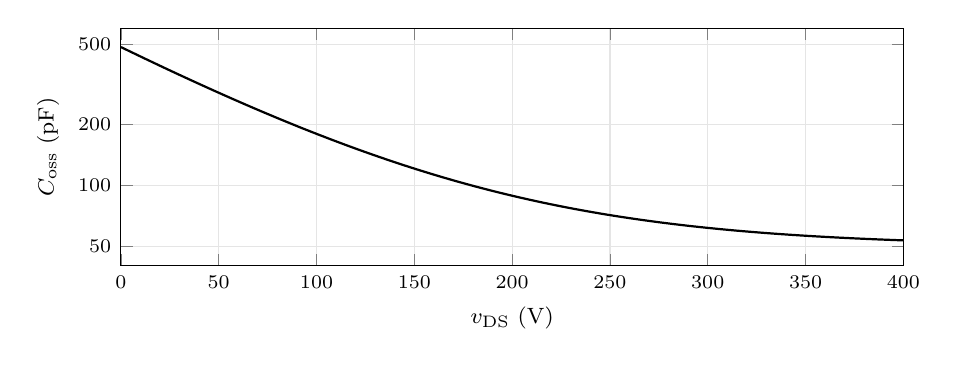
\begin{tikzpicture}
					\begin{semilogyaxis}[
							width=0.95\linewidth, height=4.6cm,
							xmin=0, xmax=400, ymin=40, ymax=600,
							xlabel={$v_\mathrm{DS}$ (V)}, ylabel={$C_\mathrm{oss}$ (pF)},
							ytick={50,100,200,500}, yticklabels={50,100,200,500},
							grid=major, grid style={gray!20},
							tick label style={font=\scriptsize}, label style={font=\footnotesize},
						]
						\addplot[black, thick, domain=0:400, samples=120] {50+434*exp(-x/83)};
					\end{semilogyaxis}
				\end{tikzpicture}
				\caption{Illustrative 650\,V GaN HEMT: $C_\mathrm{oss}=50\,\mathrm{pF}+434\,\mathrm{pF}\cdot e^{-v_\mathrm{DS}/83\,\mathrm{V}}$}
			\end{figure}
		\end{column}
		\begin{column}{0.47\textwidth}
			\begin{itemize}
				\item $C_\mathrm{oss}=C_\mathrm{DS}+C_\mathrm{GD}$ falls steeply at low voltage: by about one decade in GaN (the field plates deplete the 2DEG) and by two decades or more in Si superjunction MOSFETs (the pillars deplete).
				\item Charge and energy follow from the curve:
			\end{itemize}
			\begin{align*}
				Q_\mathrm{oss}(V) & = \int_0^V C_\mathrm{oss}(v)\,\mathrm{d}v \\
				E_\mathrm{oss}(V) & = \int_0^V v\,C_\mathrm{oss}(v)\,\mathrm{d}v
			\end{align*}
			For the model at 400\,V: $C_\mathrm{oss}=54$\,pF, $Q_\mathrm{oss}=55.7$\,nC, $E_\mathrm{oss}=6.9\,\mu$J.
		\end{column}
	\end{columns}
\end{frame}

%%%%%%%%%%%%%%%%%%%%%%%%%%%%%%%%%%%%%%%%%%%%%%%%%%%%%%%%%%%%%
%% Equivalent capacitances %%
%%%%%%%%%%%%%%%%%%%%%%%%%%%%%%%%%%%%%%%%%%%%%%%%%%%%%%%%%%%%%
\begin{frame}
	\frametitle{Equivalent output capacitances}
	Datasheets of high-voltage GaN, SiC and superjunction devices give two equivalent linear capacitances for charging from 0 to $V$ (e.g.\ 400\,V for 650\,V devices):
	\begin{table}
		\centering
		\small
		\begin{tabular}{|l|l|>{\raggedright\arraybackslash}p{5.4cm}|l|}
			\hline
			\textbf{Name}            & \textbf{Definition}                              & \textbf{Use}                                           & \textbf{Model, 400\,V} \\
			\hline
			time related $C_\mathrm{o(tr)}$   & $Q_\mathrm{oss}(V)/V$                  & charging time and charge: dead time, ZVS transition, hard turn-on loss & 139\,pF \\
			energy related $C_\mathrm{o(er)}$ & $2E_\mathrm{oss}(V)/V^2$               & stored energy                                          & 86\,pF \\
			small signal $C_\mathrm{oss}(V)$  & $\mathrm{d}Q_\mathrm{oss}/\mathrm{d}v$ at $V$ & resonance and ringing at the operating point     & 54\,pF \\
			\hline
		\end{tabular}
		\caption{Equivalent capacitances of the illustrative 650\,V device}
	\end{table}
	\begin{block}{Rule}
		For a $C_\mathrm{oss}(v)$ that falls with voltage, $C_\mathrm{oss}(V) < C_\mathrm{o(er)} < C_\mathrm{o(tr)}$. Using the small-signal value from the datasheet curve at the operating voltage underestimates both charge and energy.
	\end{block}
\end{frame}

%%%%%%%%%%%%%%%%%%%%%%%%%%%%%%%%%%%%%%%%%%%%%%%%%%%%%%%%%%%%%
%% Hard turn-on revisited %%
%%%%%%%%%%%%%%%%%%%%%%%%%%%%%%%%%%%%%%%%%%%%%%%%%%%%%%%%%%%%%
\begin{frame}
	\frametitle{Capacitive turn-on loss}
	\begin{columns}[T]
		\begin{column}{0.5\textwidth}
			\begin{figure}
				\centering
				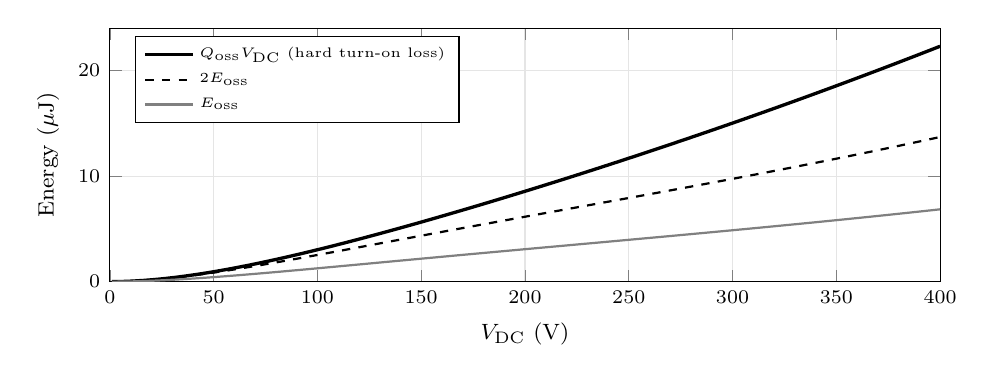
\begin{tikzpicture}
					\begin{axis}[
							width=\linewidth, height=4.8cm,
							xmin=0, xmax=400, ymin=0, ymax=24,
							xlabel={$V_\mathrm{DC}$ (V)}, ylabel={Energy ($\mu$J)},
							grid=major, grid style={gray!20},
							tick label style={font=\scriptsize}, label style={font=\footnotesize},
							legend style={font=\tiny}, legend pos=north west, legend cell align=left,
						]
						\addplot[black, very thick, domain=1:400, samples=80] {(50e-12*x+434e-12*83*(1-exp(-x/83)))*x*1e6};
						\addlegendentry{$Q_\mathrm{oss}V_\mathrm{DC}$ (hard turn-on loss)}
						\addplot[black, thick, dashed, domain=1:400, samples=80] {2*(25e-12*x^2+434e-12*83^2*(1-exp(-x/83)*(1+x/83)))*1e6};
						\addlegendentry{$2E_\mathrm{oss}$}
						\addplot[gray, thick, domain=1:400, samples=80] {(25e-12*x^2+434e-12*83^2*(1-exp(-x/83)*(1+x/83)))*1e6};
						\addlegendentry{$E_\mathrm{oss}$}
					\end{axis}
				\end{tikzpicture}
				\caption{Illustrative 650\,V GaN HEMT of the previous slides}
			\end{figure}
		\end{column}
		\begin{column}{0.47\textwidth}
			Hard turn-on in a half-bridge (Tutorial 1): $E=Q_\mathrm{oss}V_\mathrm{DC}$ for any shape of $C_\mathrm{oss}(v)$.\\[0.4em]
			Compared with the stored energy:
			\begin{equation*}
				Q_\mathrm{oss}V-2E_\mathrm{oss}=\int_0^V (V-2v)\,C_\mathrm{oss}(v)\,\mathrm{d}v \geq 0
			\end{equation*}
			if $C_\mathrm{oss}$ falls with $v$ (the weight $V-2v$ is positive where $C_\mathrm{oss}$ is large).\\[0.4em]
			At 400\,V: $Q_\mathrm{oss}V_\mathrm{DC}=22.3\,\mu$J, but $E_\mathrm{oss}=6.9\,\mu$J. An estimate based on $E_\mathrm{oss}$ is 3.3 times too optimistic.
		\end{column}
	\end{columns}
\end{frame}

%%%%%%%%%%%%%%%%%%%%%%%%%%%%%%%%%%%%%%%%%%%%%%%%%%%%%%%%%%%%%
%% Datasheet task %%
%%%%%%%%%%%%%%%%%%%%%%%%%%%%%%%%%%%%%%%%%%%%%%%%%%%%%%%%%%%%%
% Two pages: task (page 1) and task with solution (page 2).
\begin{frame}<handout:1-2>
	\frametitle{Reading a datasheet}
	\begin{columns}[T]
		\begin{column}{0.42\textwidth}
			\begin{table}
				\centering
				\small
				\begin{tabular}{|l|l|}
					\hline
					$R_\mathrm{DS(on)}$                & 5\,m$\Omega$     \\
					$Q_\mathrm{G}$ at 5\,V             & 7\,nC            \\
					$Q_\mathrm{GD}$                    & 1\,nC            \\
					$Q_\mathrm{oss}$ at 48\,V          & 25\,nC           \\
					$E_\mathrm{oss}$ at 48\,V          & 0.45\,$\mu$J     \\
					$V_\mathrm{SD}$ ($v_\mathrm{GS}=0$) & 1.8\,V          \\
					$Q_\mathrm{rr}$                    & 0                \\
					\hline
				\end{tabular}
				\caption{Illustrative 100\,V GaN transistor}
			\end{table}
		\end{column}
		\begin{column}{0.55\textwidth}
			\begin{block}{Task (5 minutes)}
				A half-bridge operates at 48\,V and 1\,MHz.
				\begin{enumerate}
					\item Calculate $C_\mathrm{o(tr)}$ and $C_\mathrm{o(er)}$.
					\item Capacitive loss with hard turn-on? What would an estimate with $E_\mathrm{oss}$ give?
					\item Minimum dead time for a ZVS transition driven by 10\,A and by 2\,A?
				\end{enumerate}
			\end{block}
		\end{column}
	\end{columns}
	\onslide<2-|handout:2>{
		\small
		\begin{enumerate}
			\item $C_\mathrm{o(tr)}=25\,\mathrm{nC}/48\,\mathrm{V}=521$\,pF, $C_\mathrm{o(er)}=2\cdot0.45\,\mu\mathrm{J}/(48\,\mathrm{V})^2=391$\,pF.
			\item $Q_\mathrm{oss}V_\mathrm{DC}f_\mathrm{sw}=1.2$\,W. With $E_\mathrm{oss}$: 0.45\,W, i.e.\ 2.7 times too low.
			\item The current moves the charge of both switches: $t_\mathrm{tr}=2Q_\mathrm{oss}/I$, i.e.\ 5\,ns at 10\,A and 25\,ns at 2\,A. A fixed dead time that works at full load is too short at light load (L8).
		\end{enumerate}
	}
\end{frame}

%%%%%%%%%%%%%%%%%%%%%%%%%%%%%%%%%%%%%%%%%%%%%%%%%%%%%%%%%%%%%
%% Coss hysteresis %%
%%%%%%%%%%%%%%%%%%%%%%%%%%%%%%%%%%%%%%%%%%%%%%%%%%%%%%%%%%%%%
\begin{frame}
	\frametitle{Output capacitance hysteresis}
	\begin{columns}[T]
		\begin{column}{0.42\textwidth}
			\begin{figure}
				\centering
				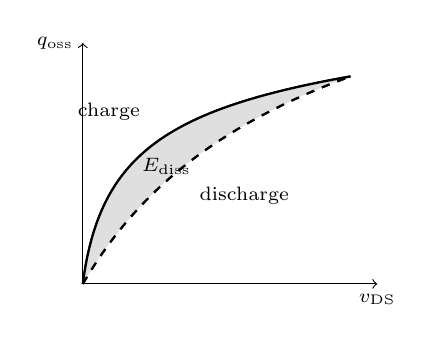
\begin{tikzpicture}[x=0.85cm, y=0.85cm, font=\scriptsize]
					\draw[->] (0,0) -- (4.4,0) node[below] {$v_\mathrm{DS}$};
					\draw[->] (0,0) -- (0,3.6) node[left] {$q_\mathrm{oss}$};
					% charging path (upper) and discharging path (lower)
					\draw[thick] (0,0) .. controls (0.25,1.9) and (1.2,2.6) .. (4,3.1);
					\draw[thick, dashed] (0,0) .. controls (0.7,1.2) and (1.8,2.3) .. (4,3.1);
					\fill[gray!25] (0,0) .. controls (0.25,1.9) and (1.2,2.6) .. (4,3.1) .. controls (1.8,2.3) and (0.7,1.2) .. (0,0);
					\draw[thick] (0,0) .. controls (0.25,1.9) and (1.2,2.6) .. (4,3.1);
					\draw[thick, dashed] (0,0) .. controls (0.7,1.2) and (1.8,2.3) .. (4,3.1);
					\node[anchor=south east] at (1.0,2.3) {charge};
					\node[anchor=north west] at (1.6,1.6) {discharge};
					\node at (1.25,1.75) {$E_\mathrm{diss}$};
				\end{tikzpicture}
				\caption{Measured charge--voltage loop (schematic); the enclosed area is the energy lost per cycle}
			\end{figure}
		\end{column}
		\begin{column}{0.55\textwidth}
			\small
			Soft switching is ideally lossless, but charging and discharging $C_\mathrm{oss}$ dissipates energy:
			\begin{itemize}
				\item reported for Si superjunction MOSFETs, GaN HEMTs and SiC diodes
				\item in GaN: equal to or greater than the conduction loss at MHz, rising exponentially with $\mathrm{d}v/\mathrm{d}t$
				\item a fixed fraction of $E_\mathrm{oss}$ is not a valid model: the loss depends on $f$, voltage swing and $\mathrm{d}v/\mathrm{d}t$
				\item within one device family the loss scales with $E_\mathrm{oss}$
			\end{itemize}
			Measured with Sawyer--Tower circuits (charge versus voltage) or calorimetrically (L5).
		\end{column}
	\end{columns}
	\blfootnote{Sources: Fedison et al., APEC 2014; Zulauf et al., IEEE TPEL, 2018; Perreault, APEC 2024 plenary.}
\end{frame}

%%%%%%%%%%%%%%%%%%%%%%%%%%%%%%%%%%%%%%%%%%%%%%%%%%%%%%%%%%%%%
%% Origin and size of Coss losses %%
%%%%%%%%%%%%%%%%%%%%%%%%%%%%%%%%%%%%%%%%%%%%%%%%%%%%%%%%%%%%%
\begin{frame}
	\frametitle{Origin and size of $C_\mathrm{oss}$ losses}
	\begin{columns}[T]
		\begin{column}{0.5\textwidth}
			\begin{figure}
				\centering
				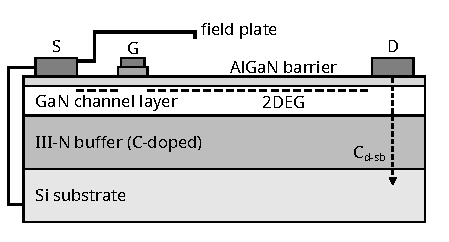
\includegraphics[width=0.92\linewidth]{fig/lec02/gan_on_si_hemt.pdf}
				\caption{Lateral GaN-on-Si HEMT (schematic, not to scale). In the device studied, up to 95\,\% of the loss came from $C_\mathrm{d\text{-}sb}$; an improved buffer cut the loss by about 70\,\%.}
			\end{figure}
		\end{column}
		\begin{column}{0.47\textwidth}
			\small
			Fit for one 650\,V GaN device (5--35\,MHz):
			\begin{equation*}
				E_\mathrm{diss}=k\,f^{\alpha}\,V_\mathrm{pp}^{\beta},\quad \alpha=0.6,\ \beta=1.7
			\end{equation*}
			\begin{table}
				\centering
				\footnotesize
				\begin{tabular}{|l|l|l|}
					\hline
					                & $E_\mathrm{diss}$ & $P=E_\mathrm{diss}f$ \\
					\hline
					10\,MHz, 400\,V & 0.12\,$\mu$J      & 1.2\,W               \\
					30\,MHz, 650\,V & 0.53\,$\mu$J      & 15.8\,W              \\
					\hline
				\end{tabular}
			\end{table}
			For comparison: 3\,A rms in 100\,m$\Omega$ give 0.9\,W. At tens of MHz, $C_\mathrm{oss}$ losses can dominate.
		\end{column}
	\end{columns}
	\blfootnote{Sources: Guacci et al., IEEE JESTPE, 2019; Zulauf et al., IEEE TPEL, 2018 (GS66504B, $k=2.84\cdot10^{-10}$, $E$ in $\mu$J).}
\end{frame}

%%%%%%%%%%%%%%%%%%%%%%%%%%%%%%%%%%%%%%%%%%%%%%%%%%%%%%%%%%%%%
%% Loss inventory %%
%%%%%%%%%%%%%%%%%%%%%%%%%%%%%%%%%%%%%%%%%%%%%%%%%%%%%%%%%%%%%
\subsection{Loss inventory at MHz}

\begin{frame}
	\frametitle{Conduction loss at MHz}
	$P_\mathrm{cond}=I_\mathrm{rms}^2\,\big(R_\mathrm{DS(on)}(T_\mathrm{j},t)+R_\mathrm{ac}(f)\big)$, with $R_\mathrm{ac}$ of package and PCB.
	\begin{itemize}
		\item $R_\mathrm{DS(on)}$ typically rises by a factor of 1.5 to 2.5 from 25\,$^\circ$C to 150\,$^\circ$C. Use the datasheet curve at the expected junction temperature.
		\item GaN HEMTs show a dynamic $R_\mathrm{DS(on)}$ (next slide).
		\item Leads and traces have skin and proximity effect at MHz (L3, L7).
		\item Soft-switching schemes often need a larger RMS current.
	\end{itemize}
	\begin{block}{Example: triangular current mode}
		A buck converter with 10\,A output current needs an inductor current between $-2$\,A and 22\,A for ZVS (L8):
		\begin{equation*}
			I_\mathrm{rms}=\sqrt{I_\mathrm{avg}^2+\Delta I^2/12}=\sqrt{10^2+24^2/12}\,\mathrm{A}=12.2\,\mathrm{A}
		\end{equation*}
		The conduction loss is 48\,\% higher than with a small ripple.
	\end{block}
\end{frame}

%%%%%%%%%%%%%%%%%%%%%%%%%%%%%%%%%%%%%%%%%%%%%%%%%%%%%%%%%%%%%
%% Dynamic Ron %%
%%%%%%%%%%%%%%%%%%%%%%%%%%%%%%%%%%%%%%%%%%%%%%%%%%%%%%%%%%%%%
\begin{frame}
	\frametitle{Dynamic on-resistance of GaN}
	\begin{columns}[T]
		\begin{column}{0.42\textwidth}
			\begin{figure}
				\centering
				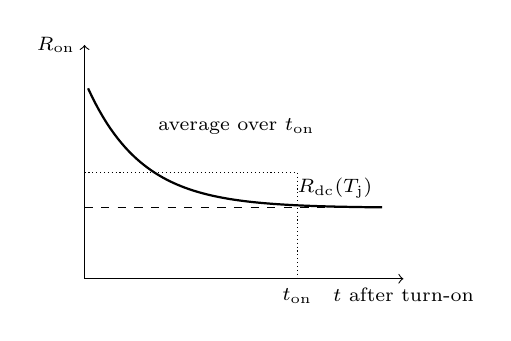
\begin{tikzpicture}[x=0.9cm, y=0.9cm, font=\scriptsize]
					\draw[->] (0,0) -- (4.5,0) node[below] {$t$ after turn-on};
					\draw[->] (0,0) -- (0,3.3) node[left] {$R_\mathrm{on}$};
					\draw[dashed] (0,1) -- (4.2,1) node[above left] {$R_\mathrm{dc}(T_\mathrm{j})$};
					\draw[thick, domain=0.05:4.2, samples=80] plot (\x, {1+1.8*exp(-1.3*\x)});
					\draw[densely dotted] (0,1.5) -- (3,1.5) -- (3,0);
					\node[anchor=north] at (3,0) {$t_\mathrm{on}$};
					\node[anchor=south west] at (0.9,1.9) {average over $t_\mathrm{on}$};
				\end{tikzpicture}
				\caption{Dynamic on-resistance after turn-on (schematic)}
			\end{figure}
		\end{column}
		\begin{column}{0.55\textwidth}
			\small
			Electrons trapped in the buffer, in the channel layer or at the surface reduce the 2DEG density for some time after turn-on.
			\begin{itemize}
				\item \textbf{Off-state trapping} grows with blocking voltage and blocking time.
				\item \textbf{Hot-electron trapping} occurs during hard turn-on. To first order it is absent with soft switching.
				\item Traps accumulate over many cycles. A double-pulse test therefore underestimates the effect; measure in continuous operation (L5).
			\end{itemize}
			Published values for 600/650\,V devices range from negligible to five to eight times $R_\mathrm{dc}$. For the device measured by Zulauf et al.\ the worst case was about $2R_\mathrm{dc}$.
		\end{column}
	\end{columns}
	\blfootnote{Source: Zulauf, Guacci, Kolar, IEEE TPEL, vol. 35, no. 6, 2020.}
\end{frame}

%%%%%%%%%%%%%%%%%%%%%%%%%%%%%%%%%%%%%%%%%%%%%%%%%%%%%%%%%%%%%
%% Turn-off with capacitive snubbing %%
%%%%%%%%%%%%%%%%%%%%%%%%%%%%%%%%%%%%%%%%%%%%%%%%%%%%%%%%%%%%%
\begin{frame}
	\frametitle{Turn-off with output capacitance}
	\begin{columns}[T]
		\begin{column}{0.45\textwidth}
			\begin{figure}
				\centering
				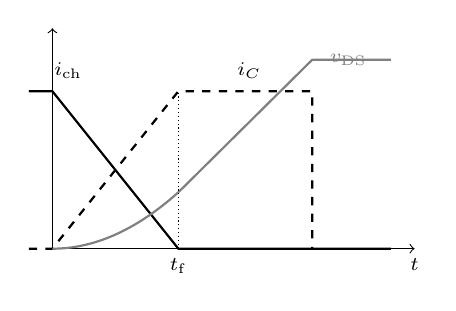
\begin{tikzpicture}[x=1.0cm, y=0.8cm, font=\scriptsize]
					\draw[->] (0,0) -- (4.6,0) node[below] {$t$};
					\draw[->] (0,0) -- (0,3.5);
					% channel current falls linearly within t_f
					\draw[thick] (-0.3,2.5) -- (0,2.5) -- (1.6,0) -- (4.3,0);
					\node[anchor=south] at (0.2,2.55) {$i_\mathrm{ch}$};
					% capacitor current rises to I
					\draw[thick, dashed] (-0.3,0) -- (0,0) -- (1.6,2.5) -- (3.3,2.5) -- (3.3,0);
					\node[anchor=south] at (2.5,2.55) {$i_C$};
					% voltage: parabola during t_f, then linear
					\draw[thick, gray, domain=0:1.6, samples=40] plot (\x, {0.35*\x*\x});
					\draw[thick, gray] (1.6,0.896) -- (3.3,3.0) -- (4.3,3.0);
					\node[anchor=west, gray] at (3.4,3.0) {$v_\mathrm{DS}$};
					\draw[densely dotted] (1.6,0) -- (1.6,2.5);
					\node[anchor=north] at (1.6,0) {$t_\mathrm{f}$};
				\end{tikzpicture}
				\caption{Turn-off of a constant current $I$ with a capacitance $C$ across the switch node}
			\end{figure}
		\end{column}
		\begin{column}{0.52\textwidth}
			If the channel current falls linearly within $t_\mathrm{f}$, the rest of the current charges $C$ and the voltage rises slowly:
			\begin{equation*}
				E_\mathrm{off}=\int_0^{t_\mathrm{f}} v_\mathrm{DS}\,i_\mathrm{ch}\,\mathrm{d}t=\frac{I^2t_\mathrm{f}^2}{24\,C}
				\quad\text{for}\quad \frac{I\,t_\mathrm{f}}{2C}<V_\mathrm{DC}
			\end{equation*}
			$C$ is the total switch-node capacitance (both $C_\mathrm{oss}$ and parasitics).\\[0.4em]
			Example: $I=10$\,A, $t_\mathrm{f}=2$\,ns, $C=400$\,pF gives 42\,nJ, compared with $\frac12 V_\mathrm{DC}It_\mathrm{f}=480$\,nJ at 48\,V.
			\begin{block}{Key message}
				A fast channel turn-off is almost lossless. Extra capacitance helps the turn-off but increases the loss of a hard turn-on.
			\end{block}
		\end{column}
	\end{columns}
\end{frame}

%%%%%%%%%%%%%%%%%%%%%%%%%%%%%%%%%%%%%%%%%%%%%%%%%%%%%%%%%%%%%
%% Reverse conduction and recovery %%
%%%%%%%%%%%%%%%%%%%%%%%%%%%%%%%%%%%%%%%%%%%%%%%%%%%%%%%%%%%%%
\begin{frame}
	\frametitle{Reverse conduction and recovery}
	\begin{table}
		\centering
		\footnotesize
		\begin{tabular}{|l|>{\raggedright\arraybackslash}p{3.4cm}|>{\raggedright\arraybackslash}p{4.0cm}|>{\raggedright\arraybackslash}p{3.2cm}|}
			\hline
			                   & \textbf{Si MOSFET}             & \textbf{e-mode GaN HEMT}                                          & \textbf{SiC MOSFET}          \\
			\hline
			Reverse path       & p--n body diode                & channel, opened by $v_\mathrm{GD}>V_\mathrm{th}$                  & p--n body diode              \\
			$V_\mathrm{SD}$    & about 0.7--1\,V                & about 1.5--3\,V (current dependent), plus $|v_\mathrm{GS,off}|$ for negative gate bias & about 3\,V or more (SiC junction) \\
			Recovery charge    & large (minority carriers)      & none                                                              & small                        \\
			\hline
		\end{tabular}
		\caption{Third-quadrant conduction during the dead time}
	\end{table}
	\begin{itemize}
		\item Datasheets: 100\,V Si MOSFET (6\,m$\Omega$) $Q_\mathrm{rr}=109$\,nC at 100\,A/$\mu$s; 100\,V GaN (7\,m$\Omega$) $V_\mathrm{SD}=1.7$\,V at 0.5\,A, no $Q_\mathrm{rr}$.
		\item $V_\mathrm{SD}$ of GaN rises by 1\,V for $v_\mathrm{GS,off}=-1$\,V and rises with temperature.
		\item Hard turn-on against a recovering Si diode costs about $Q_\mathrm{rr}V_\mathrm{DC}$; $Q_\mathrm{rr}$ grows with $\mathrm{d}i/\mathrm{d}t$ and temperature.
	\end{itemize}
	\blfootnote{Source: Lidow et al., GaN Transistors for Efficient Power Conversion, 3rd ed., 2019, Sec. 2.6 (EPC2045, BSC060N10NS3\,G).}
\end{frame}

%%%%%%%%%%%%%%%%%%%%%%%%%%%%%%%%%%%%%%%%%%%%%%%%%%%%%%%%%%%%%
%% Your turn: dead-time loss %%
%%%%%%%%%%%%%%%%%%%%%%%%%%%%%%%%%%%%%%%%%%%%%%%%%%%%%%%%%%%%%
% Two pages: task (page 1) and task with solution (page 2).
\begin{frame}<handout:1-2>
	\frametitle{Dead-time loss}
	\begin{block}{Task (3 minutes)}
		A GaN half-bridge switches 10\,A at 2\,MHz. During each of the two dead times per period ($t_\mathrm{d}=10$\,ns) the current flows in reverse through the GaN channel with $V_\mathrm{SD}=2.5$\,V.
		\begin{enumerate}
			\item Calculate the dead-time loss.
			\item How can it be reduced?
		\end{enumerate}
	\end{block}
	\onslide<2-|handout:2>{
		\begin{enumerate}
			\item $P_\mathrm{dt}=2\,V_\mathrm{SD}\,I\,t_\mathrm{d}\,f_\mathrm{sw}=2\cdot2.5\,\mathrm{V}\cdot10\,\mathrm{A}\cdot10\,\mathrm{ns}\cdot2\,\mathrm{MHz}=1$\,W.
			\item \begin{itemize}
				      \item Make the dead time only as long as the voltage transition, $2Q_\mathrm{oss}/I$ (adaptive dead time, L4).
				      \item Turn the GaN transistor off with 0\,V instead of a negative voltage, if the gate loop allows it.
				      \item A parallel Schottky diode lowers $V_\mathrm{SD}$, but adds its capacitance to the switch node.
			      \end{itemize}
		\end{enumerate}
	}
\end{frame}

%%%%%%%%%%%%%%%%%%%%%%%%%%%%%%%%%%%%%%%%%%%%%%%%%%%%%%%%%%%%%
%% Gate-drive loss %%
%%%%%%%%%%%%%%%%%%%%%%%%%%%%%%%%%%%%%%%%%%%%%%%%%%%%%%%%%%%%%
\begin{frame}
	\frametitle{Gate-drive loss}
	\begin{columns}[T]
		\begin{column}{0.45\textwidth}
			\begin{figure}
				\centering
				\begin{circuitikz}[scale=0.8, transform shape]
					\draw (0,0) to[V, l=$V_\mathrm{dr}$] (0,2.4) to[R, l=$R_\mathrm{dr}$] (2.2,2.4) to[R, l=$R_\mathrm{G,ext}$] (4.4,2.4) to[R, l=$R_\mathrm{G,int}$] (4.4,0.9) to[C, l=$C_\mathrm{iss}$] (4.4,-0.6) -- (4.4,-0.6) -- (0,-0.6) -- (0,0);
				\end{circuitikz}
				\caption{Gate loop: driver output resistance, external and internal gate resistance}
			\end{figure}
		\end{column}
		\begin{column}{0.52\textwidth}
			Charging and discharging the gate draws $P_\mathrm{G}=Q_\mathrm{G}\,V_\mathrm{dr}\,f_\mathrm{sw}$ per switch from the driver supply. It is dissipated in $R_\mathrm{dr}$, $R_\mathrm{G,ext}$ and $R_\mathrm{G,int}$ in proportion to their values; the total does not depend on $R_\mathrm{G}$.
			\begin{itemize}
				\item Use $Q_\mathrm{G}$ at $V_\mathrm{dr}$ from the gate-charge curve.
				\item 100\,V GaN, 7\,nC at 5\,V: 0.35\,W per switch at 10\,MHz.
				\item 100\,V Si, 35\,nC at 10\,V: 0.35\,W per switch at 1\,MHz.
				\item Driver quiescent and level-shifter losses also grow with $f_\mathrm{sw}$. Resonant gate drivers recover part of the energy (L4).
			\end{itemize}
		\end{column}
	\end{columns}
\end{frame}

%%%%%%%%%%%%%%%%%%%%%%%%%%%%%%%%%%%%%%%%%%%%%%%%%%%%%%%%%%%%%
%% Si versus GaN at 48 V %%
%%%%%%%%%%%%%%%%%%%%%%%%%%%%%%%%%%%%%%%%%%%%%%%%%%%%%%%%%%%%%
\begin{frame}
	\frametitle{Silicon versus GaN at 48\,V}
	\begin{columns}[T]
		\begin{column}{0.52\textwidth}
			\begin{figure}
				\centering
				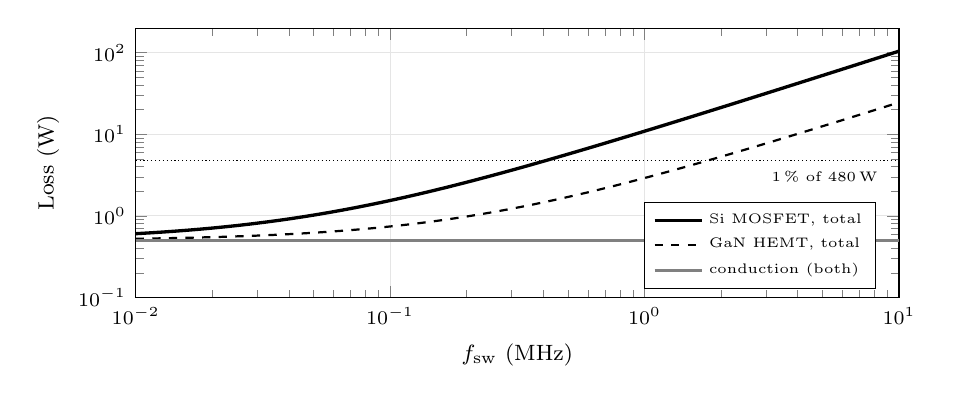
\begin{tikzpicture}
					\begin{loglogaxis}[
							width=0.93\linewidth, height=5.0cm,
							xmin=0.01, xmax=10, ymin=0.1, ymax=200,
							xlabel={$f_\mathrm{sw}$ (MHz)}, ylabel={Loss (W)},
							grid=major, grid style={gray!20},
							tick label style={font=\scriptsize}, label style={font=\footnotesize},
							legend style={font=\tiny}, legend pos=south east, legend cell align=left,
						]
						\addplot[black, very thick, domain=-2:1, samples=60] ({10^x}, {0.5+10.42*10^x});
						\addlegendentry{Si MOSFET, total}
						\addplot[black, thick, dashed, domain=-2:1, samples=60] ({10^x}, {0.5+2.41*10^x});
						\addlegendentry{GaN HEMT, total}
						\addplot[gray, thick, domain=-2:1, samples=2] ({10^x}, {0.5});
						\addlegendentry{conduction (both)}
						\addplot[black, densely dotted, domain=-2:1, samples=2, forget plot] ({10^x}, {4.8});
						\node[font=\tiny, anchor=north east] at (axis cs:9,4.6) {1\,\% of 480\,W};
					\end{loglogaxis}
				\end{tikzpicture}
				\caption{Hard-switched half-bridge, 48\,V, 10\,A, illustrative device values}
			\end{figure}
		\end{column}
		\begin{column}{0.45\textwidth}
			\footnotesize
			\begin{tabular}{|l|r|r|}
				\hline
				Energy per period ($\mu$J)                & Si    & GaN  \\
				\hline
				$Q_\mathrm{oss}V_\mathrm{DC}$             & 2.88  & 1.20 \\
				$V$--$I$ overlap                          & 3.60  & 0.96 \\
				$Q_\mathrm{rr}V_\mathrm{DC}$              & 2.88  & 0    \\
				dead time                                 & 0.36  & 0.18 \\
				gate, two switches                        & 0.70  & 0.07 \\
				\hline
				sum                                       & 10.42 & 2.41 \\
				\hline
			\end{tabular}\\[0.5em]
			Assumed: $R_\mathrm{DS(on)}=5$\,m$\Omega$ for both. Si: $Q_\mathrm{oss}=60$\,nC, $t_\mathrm{r}+t_\mathrm{f}=15$\,ns, $Q_\mathrm{rr}=60$\,nC, $Q_\mathrm{G}=35$\,nC at 10\,V, $t_\mathrm{d}=20$\,ns. GaN: values of the datasheet task, $t_\mathrm{r}+t_\mathrm{f}=4$\,ns, $t_\mathrm{d}=5$\,ns.\\[0.5em]
			Switching loss equals conduction loss at 48\,kHz (Si) and 210\,kHz (GaN). The total loss reaches 1\,\% of the output power at 0.41\,MHz and 1.8\,MHz.
		\end{column}
	\end{columns}
\end{frame}

%%%%%%%%%%%%%%%%%%%%%%%%%%%%%%%%%%%%%%%%%%%%%%%%%%%%%%%%%%%%%
%% Poll: dominant loss %%
%%%%%%%%%%%%%%%%%%%%%%%%%%%%%%%%%%%%%%%%%%%%%%%%%%%%%%%%%%%%%
% Two pages: question (page 1) and answer (page 2).
\begin{frame}<handout:1-2>
	\frametitle{Dominant loss at 5\,MHz}
	The GaN half-bridge of the previous slide is hard switched at 5\,MHz. Which loss is the largest? Vote and justify in one sentence.
	\begin{enumerate}[(a)]
		\item conduction
		\item gate drive
		\item $Q_\mathrm{oss}V_\mathrm{DC}$
		\item $V$--$I$ overlap
		\item dead time
	\end{enumerate}
	\onslide<2-|handout:2>{
		\begin{block}{Answer: (c)}
			At 5\,MHz: $Q_\mathrm{oss}V_\mathrm{DC}$ 6.0\,W, overlap 4.8\,W, dead time 0.9\,W, conduction 0.5\,W, gate 0.35\,W; total 12.6\,W or 2.6\,\% of 480\,W. A stronger gate driver only reduces the overlap term. The capacitive term requires zero-voltage switching.
		\end{block}
	}
\end{frame}

%%%%%%%%%%%%%%%%%%%%%%%%%%%%%%%%%%%%%%%%%%%%%%%%%%%%%%%%%%%%%
%% Hard versus soft switching %%
%%%%%%%%%%%%%%%%%%%%%%%%%%%%%%%%%%%%%%%%%%%%%%%%%%%%%%%%%%%%%
\subsection{Hard versus soft switching}

\begin{frame}
	\frametitle{Soft-switching techniques}
	\begin{table}
		\centering
		\small
		\begin{tabular}{|>{\raggedright\arraybackslash}p{2.9cm}|>{\raggedright\arraybackslash}p{4.4cm}|>{\raggedright\arraybackslash}p{4.9cm}|}
			\hline
			\textbf{Technique}                    & \textbf{Removes}                                                          & \textbf{Remains}                                                                    \\
			\hline
			Zero-voltage switching (ZVS) at turn-on & $Q_\mathrm{oss}V_\mathrm{DC}$, turn-on overlap, reverse recovery          & turn-off overlap (small with $C_\mathrm{oss}$), $C_\mathrm{oss}$ hysteresis, gate drive, dead-time conduction, larger RMS current \\
			\hline
			Zero-current switching (ZCS) at turn-off & turn-off overlap, tail current (IGBT)                                    & $Q_\mathrm{oss}V_\mathrm{DC}$ at turn-on, unless the voltage is also zero              \\
			\hline
			Auxiliary circuits (ZVT, ZCT)         & as ZVS or ZCS for the main switch                                         & losses and complexity of the auxiliary switch                                       \\
			\hline
		\end{tabular}
		\caption{Which loss terms are removed by soft switching}
	\end{table}
	\begin{itemize}
		\item MOSFETs and GaN HEMTs need ZVS: their main loss is the capacitive turn-on loss, which ZCS does not remove.
		\item ZVS needs an inductive current that commutates the switch node within the dead time (L8--L10).
	\end{itemize}
\end{frame}

%%%%%%%%%%%%%%%%%%%%%%%%%%%%%%%%%%%%%%%%%%%%%%%%%%%%%%%%%%%%%
%% Poll: larger die %%
%%%%%%%%%%%%%%%%%%%%%%%%%%%%%%%%%%%%%%%%%%%%%%%%%%%%%%%%%%%%%
% Two pages: question (page 1) and answer (page 2).
\begin{frame}<handout:1-2>
	\frametitle{Larger die, lower loss?}
	You replace the GaN transistor of the 48\,V half-bridge by one with twice the die area, i.e.\ half the $R_\mathrm{DS(on)}$ and twice all charges. Does the loss go down? Vote: yes, no, it depends.
	\onslide<2-|handout:2>{
		\begin{block}{Answer: it depends on $f_\mathrm{sw}$}
			Conduction loss halves, all charge-related losses double:
			\begin{itemize}
				\item 100\,kHz: $0.5+0.24\,\mathrm{W}\rightarrow 0.25+0.48\,\mathrm{W}$, practically no change.
				\item 1\,MHz: $0.5+2.41\,\mathrm{W}\rightarrow 0.25+4.82\,\mathrm{W}$, the loss rises by 74\,\%.
			\end{itemize}
			Above a certain frequency a smaller die is better. The next slide finds the optimum.
		\end{block}
	}
\end{frame}

%%%%%%%%%%%%%%%%%%%%%%%%%%%%%%%%%%%%%%%%%%%%%%%%%%%%%%%%%%%%%
%% Optimum die size %%
%%%%%%%%%%%%%%%%%%%%%%%%%%%%%%%%%%%%%%%%%%%%%%%%%%%%%%%%%%%%%
\begin{frame}
	\frametitle{Optimum die size}
	\begin{columns}[T]
		\begin{column}{0.5\textwidth}
			\begin{figure}
				\centering
				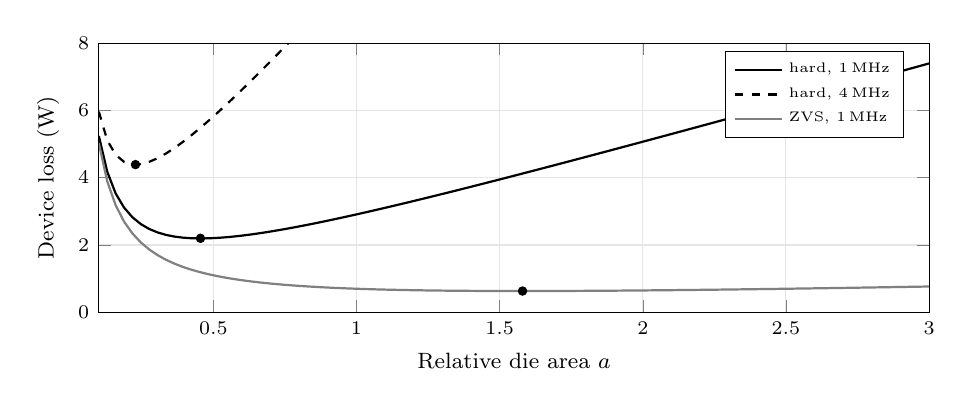
\begin{tikzpicture}
					\begin{axis}[
							width=\linewidth, height=5.0cm,
							xmin=0.1, xmax=3, ymin=0, ymax=8,
							xlabel={Relative die area $a$}, ylabel={Device loss (W)},
							grid=major, grid style={gray!20},
							tick label style={font=\scriptsize}, label style={font=\footnotesize},
							legend style={font=\tiny}, legend pos=north east, legend cell align=left,
						]
						\addplot[black, thick, domain=0.1:3, samples=100] {0.5/x+2.41*x};
						\addlegendentry{hard, 1\,MHz}
						\addplot[black, thick, dashed, domain=0.1:3, samples=100] {0.5/x+2.41*4*x};
						\addlegendentry{hard, 4\,MHz}
						\addplot[gray, thick, domain=0.1:3, samples=100] {0.5/x+0.2*x};
						\addlegendentry{ZVS, 1\,MHz}
						\addplot[only marks, mark=*, mark size=1.5pt, forget plot] coordinates {(0.455,2.20) (0.228,4.39) (1.58,0.632)};
					\end{axis}
				\end{tikzpicture}
				\caption{48\,V, 10\,A half-bridge; $a=1$ is the GaN device of the previous slides; ZVS: 0.2\,$\mu$J per period remain}
			\end{figure}
		\end{column}
		\begin{column}{0.47\textwidth}
			\small With die area $a$: $R_\mathrm{DS(on)}=R_1/a$, energy per period $E_1\,a$:
			\begin{gather*}
				P(a)=\frac{I_\mathrm{rms}^2R_1}{a}+E_1\,a\,f_\mathrm{sw}\\
				a_\mathrm{opt}=I_\mathrm{rms}\sqrt{R_1/(E_1f_\mathrm{sw})}\\
				P_\mathrm{min}=2I_\mathrm{rms}\sqrt{R_1E_1f_\mathrm{sw}}
			\end{gather*}
			\begin{itemize}
				\item At the optimum, conduction loss equals switching loss.
				\item $P_\mathrm{min}\propto\sqrt{f_\mathrm{sw}}$ and $\propto\sqrt{R_1E_1}$, the root of a figure of merit.
				\item Soft switching lowers $E_1$: larger die, lower loss.
			\end{itemize}
		\end{column}
	\end{columns}
\end{frame}

%%%%%%%%%%%%%%%%%%%%%%%%%%%%%%%%%%%%%%%%%%%%%%%%%%%%%%%%%%%%%
%% Devices %%
%%%%%%%%%%%%%%%%%%%%%%%%%%%%%%%%%%%%%%%%%%%%%%%%%%%%%%%%%%%%%
\subsection{Devices for high frequency}

\begin{frame}
	\frametitle{Devices up to 100\,V}
	\begin{table}
		\centering
		\small
		\begin{tabular}{|l|>{\raggedright\arraybackslash}p{4.9cm}|>{\raggedright\arraybackslash}p{5.5cm}|}
			\hline
			                       & \textbf{Si trench / shielded-gate MOSFET}        & \textbf{e-mode GaN HEMT}                              \\
			\hline
			Structure              & vertical                                         & lateral, all contacts on top                          \\
			Gate drive             & 10\,V, robust ($\pm20$\,V)                       & 5\,V, absolute maximum about $+6/-4$\,V                \\
			Charges per $R_\mathrm{DS(on)}$ & reference                               & several times lower $Q_\mathrm{G}$, $Q_\mathrm{GD}$, $Q_\mathrm{oss}$ \\
			Reverse recovery       & yes                                              & none                                                  \\
			Package                & QFN, power stages with driver                    & chip-scale LGA/BGA, package inductance of a few hundred pH \\
			\hline
		\end{tabular}
		\caption{Low-voltage device technologies}
	\end{table}
	\begin{itemize}
		\item Trend to integration: Si power stages, monolithic GaN power ICs.
		\item At 48\,V and several MHz GaN is the usual choice; at 12\,V below 1\,MHz Si power stages remain competitive.
	\end{itemize}
	\blfootnote{Sources: Lidow et al., 2019; Reusch and Strydom, IEEE TPEL, 2014.}
\end{frame}

%%%%%%%%%%%%%%%%%%%%%%%%%%%%%%%%%%%%%%%%%%%%%%%%%%%%%%%%%%%%%
%% High-voltage devices %%
%%%%%%%%%%%%%%%%%%%%%%%%%%%%%%%%%%%%%%%%%%%%%%%%%%%%%%%%%%%%%
\begin{frame}
	\frametitle{Devices for 600--650\,V}
	\begin{table}
		\centering
		\small
		\begin{tabular}{|l|>{\raggedright\arraybackslash}p{9.6cm}|}
			\hline
			Si superjunction MOSFET & cheap and robust, but large $Q_\mathrm{rr}$, strongly nonlinear $C_\mathrm{oss}$ with large $Q_\mathrm{oss}$ and hysteresis; mainly below a few hundred kHz \\
			e-mode GaN (p-GaN gate) & lowest charges, no $Q_\mathrm{rr}$; sensitive gate (low $V_\mathrm{th}$, limited gate voltage), dynamic $R_\mathrm{DS(on)}$, $C_\mathrm{oss}$ losses at MHz \\
			Cascode GaN             & normally-on GaN with a low-voltage Si MOSFET, robust gate; the Si MOSFET adds charge and a recovery effect \\
			SiC MOSFET              & high temperature capability and avalanche robustness; larger charges and 15--18\,V gate drive; body diode with high $V_\mathrm{SD}$ \\
			\hline
		\end{tabular}
		\caption{High-voltage device technologies for switching at hundreds of kHz to MHz}
	\end{table}
	\begin{itemize}
		\item The $C_\mathrm{oss}$ loss ranking depends on the voltage swing: in one study the cascode device had lower losses below 300\,V, the e-mode devices above.
		\item Choose by voltage, switching mode (hard or soft) and frequency, then compare complete loss budgets (Tutorial 2).
	\end{itemize}
	\blfootnote{Source: Zulauf et al., IEEE TPEL, vol. 33, no. 12, 2018.}
\end{frame}

%%%%%%%%%%%%%%%%%%%%%%%%%%%%%%%%%%%%%%%%%%%%%%%%%%%%%%%%%%%%%
%% Common-source inductance %%
%%%%%%%%%%%%%%%%%%%%%%%%%%%%%%%%%%%%%%%%%%%%%%%%%%%%%%%%%%%%%
\begin{frame}
	\frametitle{Common-source inductance}
	\begin{columns}[T]
		\begin{column}{0.48\textwidth}
			\begin{figure}
				\centering
				\begin{circuitikz}[scale=0.8, transform shape]
					\draw (3,2) node[nigfete](T){};
					\draw (T.D) -- ++(0,0.6) node[above] {drain};
					\draw (T.S) to[L, l_=$L_\mathrm{CS}$] (3,-0.6) coordinate (s) -- ++(0,-0.4) node[below] {power source};
					\draw (T.G) -- ++(-0.4,0) coordinate (g) to[R, l_=$R_\mathrm{G}$] ($(g)+(-1.6,0)$) coordinate (d) to[sV, l_=driver] (d |- s) -- (s);
					\draw (s) node[circ]{};
					\draw[->] (3.5,1.5) -- (3.5,0.3) node[midway, right] {$i_\mathrm{D}$};
				\end{circuitikz}
				\caption{The inductance $L_\mathrm{CS}$ is common to the power loop and the gate loop}
			\end{figure}
		\end{column}
		\begin{column}{0.49\textwidth}
			\small
			During the current transitions $L_\mathrm{CS}$ induces a voltage that opposes the gate drive:
			\begin{equation*}
				v_\mathrm{GS}=v_\mathrm{dr}-R_\mathrm{G}i_\mathrm{G}-L_\mathrm{CS}\frac{\mathrm{d}i_\mathrm{D}}{\mathrm{d}t}
			\end{equation*}
			1\,nH at 5\,A/ns gives 5\,V, as much as the whole GaN gate drive voltage.
			\begin{itemize}
				\item slower current transitions, more overlap loss
				\item calculated for a GaN buck: 1\,nH of $L_\mathrm{CS}$ adds 50\,\% loss (Reusch and Strydom)
				\item remedy: Kelvin-source pin for the gate loop, low-inductance package
			\end{itemize}
		\end{column}
	\end{columns}
	\blfootnote{Sources: Lidow et al., 2019, Sec. 3.6.1 and 7.3.1; Reusch and Strydom, IEEE TPEL, vol. 29, no. 4, 2014.}
\end{frame}

%%%%%%%%%%%%%%%%%%%%%%%%%%%%%%%%%%%%%%%%%%%%%%%%%%%%%%%%%%%%%
%% Datasheet limits %%
%%%%%%%%%%%%%%%%%%%%%%%%%%%%%%%%%%%%%%%%%%%%%%%%%%%%%%%%%%%%%
\begin{frame}
	\frametitle{What datasheets do not show}
	\begin{columns}[T]
		\begin{column}{0.48\textwidth}
			\textbf{Usually given}
			\begin{itemize}
				\item $R_\mathrm{DS(on)}$ versus temperature
				\item $Q_\mathrm{G}$, $Q_\mathrm{GS}$, $Q_\mathrm{GD}$ and the gate-charge curve
				\item $C_\mathrm{oss}(v)$, $Q_\mathrm{oss}$, $E_\mathrm{oss}$, $C_\mathrm{o(tr)}$, $C_\mathrm{o(er)}$
				\item $V_\mathrm{SD}$ and $Q_\mathrm{rr}$ at one operating point
				\item $E_\mathrm{on}$, $E_\mathrm{off}$ from a double-pulse test on the manufacturer's board
			\end{itemize}
		\end{column}
		\begin{column}{0.48\textwidth}
			\textbf{Usually missing}
			\begin{itemize}
				\item $C_\mathrm{oss}$ hysteresis loss under soft switching
				\item dynamic $R_\mathrm{DS(on)}$ in continuous operation
				\item $Q_\mathrm{rr}$ at your $\mathrm{d}i/\mathrm{d}t$ and temperature
				\item switching energies with your layout, gate driver and loop inductance
			\end{itemize}
		\end{column}
	\end{columns}
	\begin{block}{Consequence}
		A loss budget from datasheet values is a first estimate. The missing terms must be measured in the application, which is the subject of L5.
	\end{block}
\end{frame}

%%%%%%%%%%%%%%%%%%%%%%%%%%%%%%%%%%%%%%%%%%%%%%%%%%%%%%%%%%%%%
%% Key messages %%
%%%%%%%%%%%%%%%%%%%%%%%%%%%%%%%%%%%%%%%%%%%%%%%%%%%%%%%%%%%%%
\begin{frame}
	\frametitle{Key messages}
	\begin{enumerate}
		\item The hard turn-on loss is $Q_\mathrm{oss}V_\mathrm{DC}$. Estimates with $E_\mathrm{oss}$ or with the small-signal $C_\mathrm{oss}$ are too optimistic.
		\item Use $C_\mathrm{o(tr)}$ for charge and time, $C_\mathrm{o(er)}$ for stored energy.
		\item Soft switching removes the capacitive turn-on loss, but $C_\mathrm{oss}$ hysteresis, gate drive, dead time and a larger RMS current remain.
		\item At the optimum die size, conduction and switching loss are equal and the total loss grows with $\sqrt{f_\mathrm{sw}}$.
		\item Low common-source and package inductance are as important as the device itself.
	\end{enumerate}
\end{frame}

%%%%%%%%%%%%%%%%%%%%%%%%%%%%%%%%%%%%%%%%%%%%%%%%%%%%%%%%%%%%%
%% Exit ticket %%
%%%%%%%%%%%%%%%%%%%%%%%%%%%%%%%%%%%%%%%%%%%%%%%%%%%%%%%%%%%%%
% Two pages: questions (page 1) and answers (page 2).
\begin{frame}<handout:1-2>
	\frametitle{Exit ticket}
	\begin{varblock}[\textwidth]{Three questions, one minute each}
		\begin{enumerate}
			\item Which equivalent capacitance gives the time of a ZVS transition?
			\item Name two losses that remain in a GaN half-bridge with perfect ZVS.
			\item The switching frequency of an optimally sized design rises from 1 to 4\,MHz. By which factor does the minimum device loss change?
		\end{enumerate}
	\end{varblock}
	\onslide<2-|handout:2>{
		\begin{enumerate}
			\item $C_\mathrm{o(tr)}=Q_\mathrm{oss}/V$, since the transition moves a charge.
			\item Any two of: $C_\mathrm{oss}$ hysteresis, gate drive, dead-time conduction, turn-off overlap, conduction with a larger RMS current.
			\item By $\sqrt{4}=2$, with a die area half as large.
		\end{enumerate}
	}
\end{frame}

%%%%%%%%%%%%%%%%%%%%%%%%%%%%%%%%%%%%%%%%%%%%%%%%%%%%%%%%%%%%%
%% References %%
%%%%%%%%%%%%%%%%%%%%%%%%%%%%%%%%%%%%%%%%%%%%%%%%%%%%%%%%%%%%%
\begin{frame}
	\frametitle{References}
	\scriptsize
	\begin{itemize}
		\item A. Lidow, M. de Rooij, J. Strydom, D. Reusch, J. Glaser, \textit{GaN Transistors for Efficient Power Conversion}, 3rd ed., Wiley, 2019.
		\item R.\,W. Erickson, D. Maksimovi\'c, \textit{Fundamentals of Power Electronics}, 3rd ed., Springer, 2020, Ch. 4.
		\item J.\,B. Fedison, M. Fornage, M.\,J. Harrison, D.\,R. Zimmanck, ``Coss related energy loss in power MOSFETs used in zero-voltage-switched applications,'' IEEE APEC 2014, pp.\ 150--156.
		\item G. Zulauf, S. Park, W. Liang, K.\,N. Surakitbovorn, J. Rivas-Davila, ``COSS losses in 600 V GaN power semiconductors in soft-switched, high- and very-high-frequency power converters,'' IEEE Trans.\ Power Electron., vol.\ 33, no.\ 12, pp.\ 10748--10763, 2018.
		\item M. Guacci et al., ``On the origin of the Coss-losses in soft-switching GaN-on-Si power HEMTs,'' IEEE J.\ Emerg.\ Sel.\ Topics Power Electron., vol.\ 7, no.\ 2, pp.\ 679--694, 2019.
		\item G. Zulauf, M. Guacci, J.\,W. Kolar, ``Dynamic on-resistance in GaN-on-Si HEMTs: Origins, dependencies, and future characterization frameworks,'' IEEE Trans.\ Power Electron., vol.\ 35, no.\ 6, pp.\ 5581--5588, 2020.
		\item D. Reusch, J. Strydom, ``Understanding the effect of PCB layout on circuit performance in a high-frequency gallium-nitride-based point of load converter,'' IEEE Trans.\ Power Electron., vol.\ 29, no.\ 4, pp.\ 2008--2015, 2014.
		\item D.\,J. Perreault, ``Opportunities, progress and challenges in high-frequency power conversion,'' plenary talk, IEEE APEC 2024.
	\end{itemize}
\end{frame}
